\chapter{Practical Evaluation and Benchmark Results}
\label{chap:practical_evaluation}

\section{Retained Security Reasoning}
\label{sec:security_proofs}

Formal reasoning remains useful because the benchmark suite validates implementation behavior, not cryptographic soundness by itself. The claims retained in this thesis are intentionally narrower than full end-to-end protocol proofs.

\textbf{Confidentiality claim.}  
If the nonce discipline is respected and the underlying AEAD schemes behave as expected, then the benchmarked data plane inherits the confidentiality properties of AES-GCM and ChaCha20-Poly1305 at the profile level.

\textbf{Authentication claim.}  
If HMAC-SHA256, the implemented sequence-bound hash-token checks, and the receiver-side replay filter behave as expected, then the benchmarked data plane can reject forged runtime packets and duplicate already accepted packets within the same epoch.

These statements should not be read as full proofs of the complete adaptive architecture described earlier. In particular, the benchmark does not validate signed control-plane messages, multi-node synchronization, or broader swarm-level trust properties. The role of this section is therefore to bound the interpretation of the benchmark: the practical evaluation targets a pairwise adaptive secure-communication prototype with retained data-plane reasoning.

\section{Benchmark Implementation and Setup}
\label{sec:benchmark_setup}

The practical evaluation uses an executable benchmark suite rather than analytical performance estimates alone. The implementation instantiates two containerized peers that exchange protected messages over gRPC. Session establishment uses X25519 with HKDF-derived epoch material. Heavy and balanced modes use AES-GCM with additional HMAC-based runtime authentication, while lightweight mode uses ChaCha20-Poly1305 with a sequence-bound hash token and receiver-side duplicate rejection within each epoch. The adaptive controller switches among these profiles according to scripted threat and energy schedules.

The final benchmark pass uses the following fixed setup:
\begin{itemize}
    \item two communicating peers on the measured data path;
    \item CPU cap of 0.05 cores per peer in the main stability sweep;
    \item memory cap of 128~MiB per peer;
    \item message size of 65\,536 bytes;
    \item experiment duration of 60 seconds;
    \item three repeats per matrix cell;
    \item rekey interval of 2 seconds in the main stability sweep.
\end{itemize}

Network impairment is disabled in the main stability sweep so that the constrained CPU budget dominates the observed behavior. Threat and energy inputs are scripted rather than sensed from physical hardware. The adaptive scenario starts in a balanced low-threat regime, escalates to heavy mode at 12 seconds, returns to balanced mode at 24 seconds, switches to lightweight mode at 36 seconds under a low-energy condition, and returns to heavy mode at 48 seconds when threat rises again.

The benchmark reports the following metrics:
\begin{itemize}
    \item measured p50, p95, and p99 message latency;
    \item achieved throughput and delivered-message count;
    \item mode switches and message-profile mix for adaptive runs;
    \item drop rate against attempted sends;
    \item normalized energy proxy per delivered message;
    \item cryptographic work per delivered message, defined as bytes processed by encryption, decryption, and authentication primitives;
    \item long-run protection-tier work and policy-fit share for switching behavior;
    \item standard deviation of throughput across repeats.
\end{itemize}

The energy values reported in this chapter are \emph{model-based proxies}, not physical power measurements. They remain useful for relative comparison across profiles under the same workload, but they must not be interpreted as battery-accurate consumption.
For the figures in this chapter, the more important cost metric is cryptographic work. Unlike the energy proxy, this is not a weighted model: it is derived from raw run counters, the message-profile mix, and the bytes processed by the implemented crypto primitives.

The final artifact directory is \path{benchmarks/thesis-report-final}. It contains 228 completed benchmark summary rows from a single benchmark pass: 84 main-stability runs, 72 CPU-sensitivity runs, 36 rekey-sensitivity runs, and 36 network-impairment runs. Every matrix cell has three completed summary rows, all comparison rows contain a \texttt{source\_run\_dir}, and the generated report includes CSV, JSON, SVG, and PNG artifacts for the comparison, sweep, CPU sensitivity, rekey sensitivity, and network impairment plots.

The repository separates source artifacts from generated evidence. The benchmark package contains the executable implementation, Docker setup, scenario presets, and tests, while \path{benchmarks/thesis-report-final} contains the curated result matrix used for the tables and figures in this chapter. The public repository for the thesis artifact is available at \url{https://github.com/mazzz3r/adaptive-swarm-crypto-thesis}.

\section{Main Stability Sweep}
\label{sec:saturation_results}

The main sweep evaluates offered rates from 25 to 300 messages per second under the same 0.05-core CPU cap. Table~\ref{tab:main_stability_sweep} reports medians across three repeats per cell, with throughput standard deviation included to show run-to-run spread.

\begin{table}[H]
\centering
\scriptsize
\caption{Main stability sweep; crypto work is in MiB per delivered message}
\label{tab:main_stability_sweep}
\renewcommand{\arraystretch}{1.15}
\resizebox{\textwidth}{!}{%
\begin{tabular}{|c|l|c|c|c|c|c|c|c|c|}
\hline
\textbf{Rate} & \textbf{Mode} & \textbf{Runs} & \textbf{Med. P50} & \textbf{Med. P95} & \textbf{Med. P99} & \textbf{Med. throughput} & \textbf{Med. drop \%} & \textbf{Med. crypto work} & \textbf{Throughput std} \\
\hline
25 & Heavy & 3 & 77.606 & 294.362 & 397.421 & 25.0 & 0.000 & 0.2500 & 0.00 \\
25 & Balanced & 3 & 12.422 & 199.912 & 298.894 & 25.0 & 0.000 & 0.2500 & 0.00 \\
25 & Lightweight & 3 & 30.701 & 202.364 & 304.612 & 25.0 & 0.000 & 0.1251 & 0.01 \\
25 & Adaptive & 3 & 25.296 & 202.027 & 301.172 & 25.0 & 0.000 & 0.2248 & 0.02 \\
50 & Heavy & 3 & 197.992 & 543.232 & 795.484 & 46.3 & 6.877 & 0.2500 & 0.35 \\
50 & Balanced & 3 & 178.694 & 695.961 & 798.890 & 47.6 & 4.447 & 0.2500 & 2.00 \\
50 & Lightweight & 3 & 101.445 & 546.791 & 699.806 & 47.7 & 4.167 & 0.1251 & 0.24 \\
50 & Adaptive & 3 & 100.938 & 695.493 & 898.012 & 46.9 & 6.175 & 0.2240 & 2.30 \\
75 & Heavy & 3 & 198.307 & 697.320 & 825.192 & 56.7 & 24.356 & 0.2500 & 0.38 \\
75 & Balanced & 3 & 101.597 & 403.873 & 701.058 & 54.1 & 26.443 & 0.2500 & 6.53 \\
75 & Lightweight & 3 & 101.698 & 596.553 & 774.667 & 57.2 & 23.489 & 0.1251 & 0.58 \\
75 & Adaptive & 3 & 141.028 & 597.793 & 798.515 & 53.7 & 27.923 & 0.2257 & 2.10 \\
100 & Heavy & 3 & 124.843 & 571.559 & 825.390 & 58.4 & 40.110 & 0.2500 & 0.79 \\
100 & Balanced & 3 & 102.750 & 500.696 & 700.531 & 59.9 & 38.484 & 0.2500 & 2.67 \\
100 & Lightweight & 3 & 128.887 & 694.480 & 800.385 & 62.7 & 36.206 & 0.1251 & 2.60 \\
100 & Adaptive & 3 & 195.263 & 599.890 & 752.292 & 61.2 & 38.783 & 0.2256 & 1.56 \\
150 & Heavy & 3 & 102.715 & 695.176 & 896.869 & 67.0 & 54.025 & 0.2500 & 2.78 \\
150 & Balanced & 3 & 196.844 & 601.281 & 798.638 & 68.0 & 54.189 & 0.2500 & 4.77 \\
150 & Lightweight & 3 & 201.109 & 601.308 & 795.585 & 56.5 & 60.181 & 0.1251 & 1.42 \\
150 & Adaptive & 3 & 103.044 & 496.674 & 699.220 & 58.7 & 58.410 & 0.2221 & 4.61 \\
200 & Heavy & 3 & 200.797 & 697.407 & 901.111 & 60.9 & 68.615 & 0.2500 & 1.30 \\
200 & Balanced & 3 & 201.448 & 797.382 & 963.524 & 61.2 & 67.627 & 0.2500 & 1.34 \\
200 & Lightweight & 3 & 198.301 & 700.638 & 896.513 & 63.9 & 67.776 & 0.1251 & 2.21 \\
200 & Adaptive & 3 & 199.721 & 699.131 & 902.077 & 59.6 & 69.764 & 0.2243 & 1.01 \\
300 & Heavy & 3 & 198.630 & 699.370 & 898.656 & 62.0 & 77.631 & 0.2500 & 1.10 \\
300 & Balanced & 3 & 200.033 & 695.980 & 895.410 & 63.1 & 78.873 & 0.2500 & 0.86 \\
300 & Lightweight & 3 & 198.126 & 795.373 & 901.518 & 61.0 & 75.341 & 0.1251 & 1.90 \\
300 & Adaptive & 3 & 199.256 & 697.619 & 899.595 & 63.7 & 78.447 & 0.2230 & 2.58 \\
\hline
\end{tabular}
}
\end{table}

\begin{figure}[H]
\centering
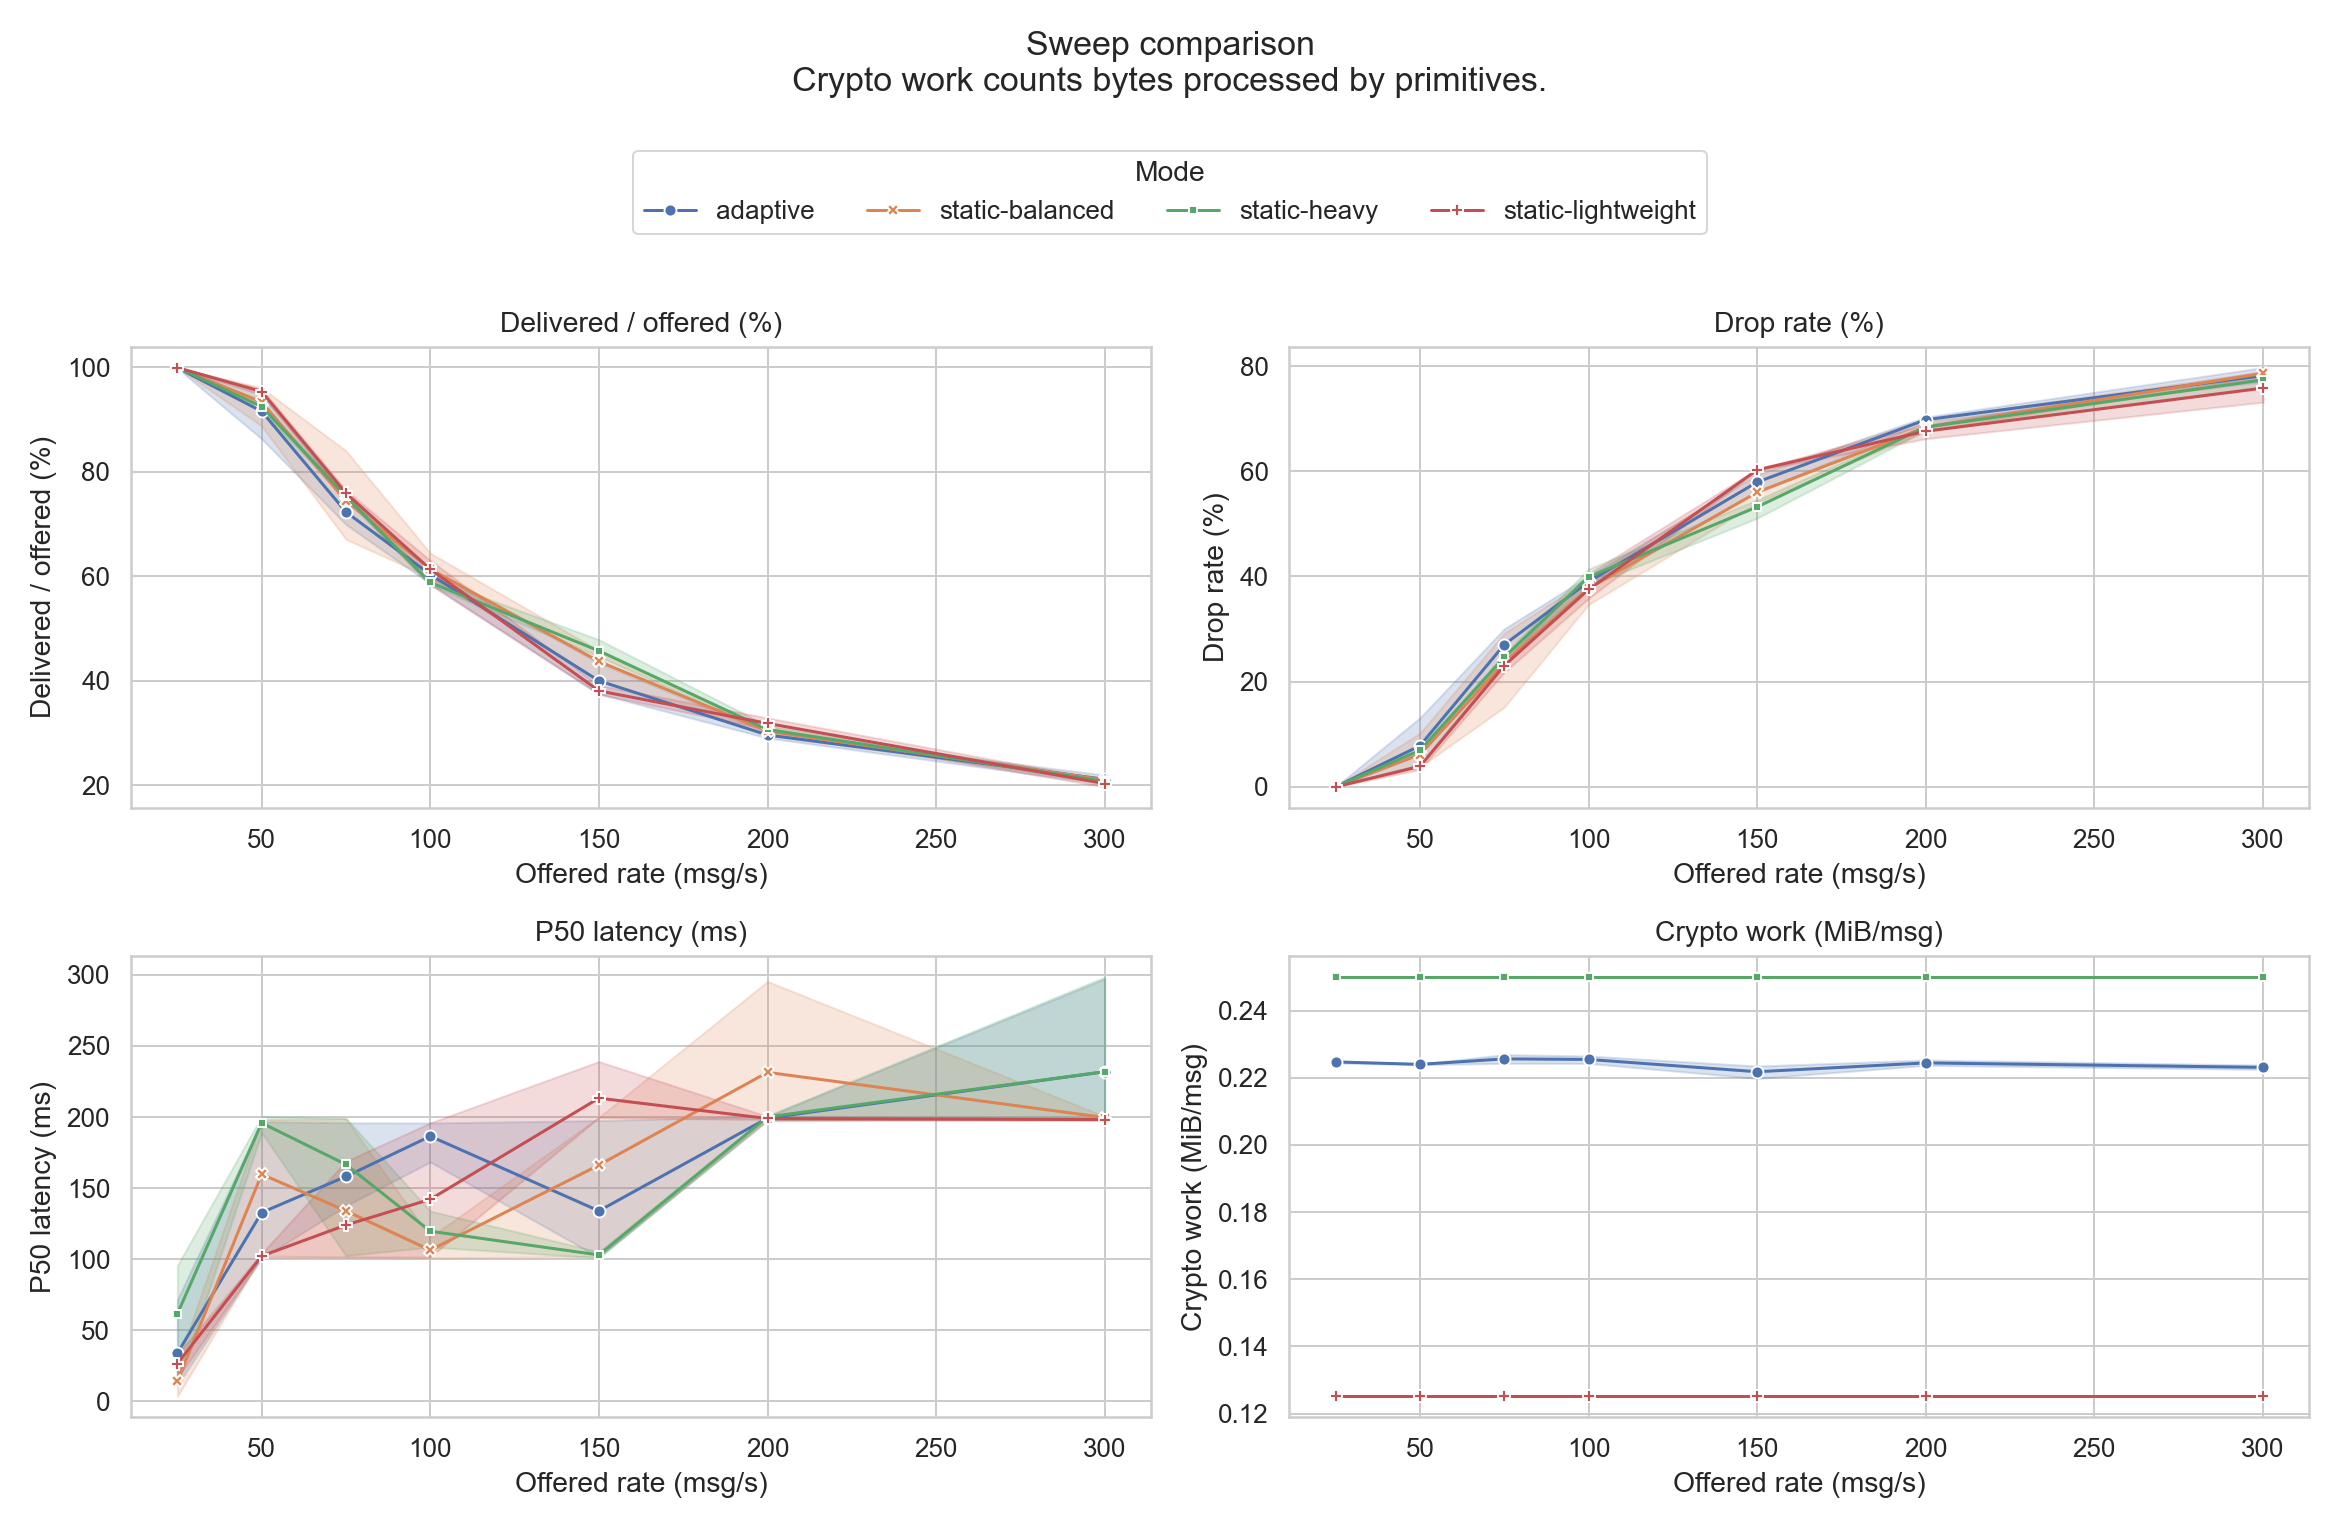
\includegraphics[width=\textwidth]{figs/benchmark_sweep_metrics.png}
\caption{Main stability sweep metrics: delivery ratio, drop rate, latency, and cryptographic work per delivered message.}
\label{fig:benchmark_sweep_metrics}
\end{figure}

The sweep shows a clear knee between 25 and 75 messages per second under the 0.05-core cap on the host system. At 25 messages per second all four strategies deliver the full offered rate. At 50 messages per second the prototype already starts dropping a small share of messages, and by 75--100 messages per second it is CPU- and queue-limited. Above that point, increasing the offered rate mostly increases sender-side drops rather than delivered throughput. Figure~\ref{fig:benchmark_sweep_metrics} makes this saturation effect explicit by plotting delivered throughput as a fraction of offered load.

The close spacing of the delivery, drop-rate, and latency curves is expected for this long-run end-to-end setup. These panels measure the whole containerized gRPC pipeline, so shared queueing, scheduling, serialization, and payload-transfer costs dominate once the run is near saturation. The profile-specific difference is therefore shown separately as cryptographic work. Heavy and balanced modes process about twice as many crypto primitive bytes per delivered message as lightweight mode because they add an HMAC authentication pass on top of AEAD encryption and decryption. Adaptive remains between the authenticated static profiles and lightweight mode because it spends only part of the run in lightweight mode.

\begin{figure}[H]
\centering
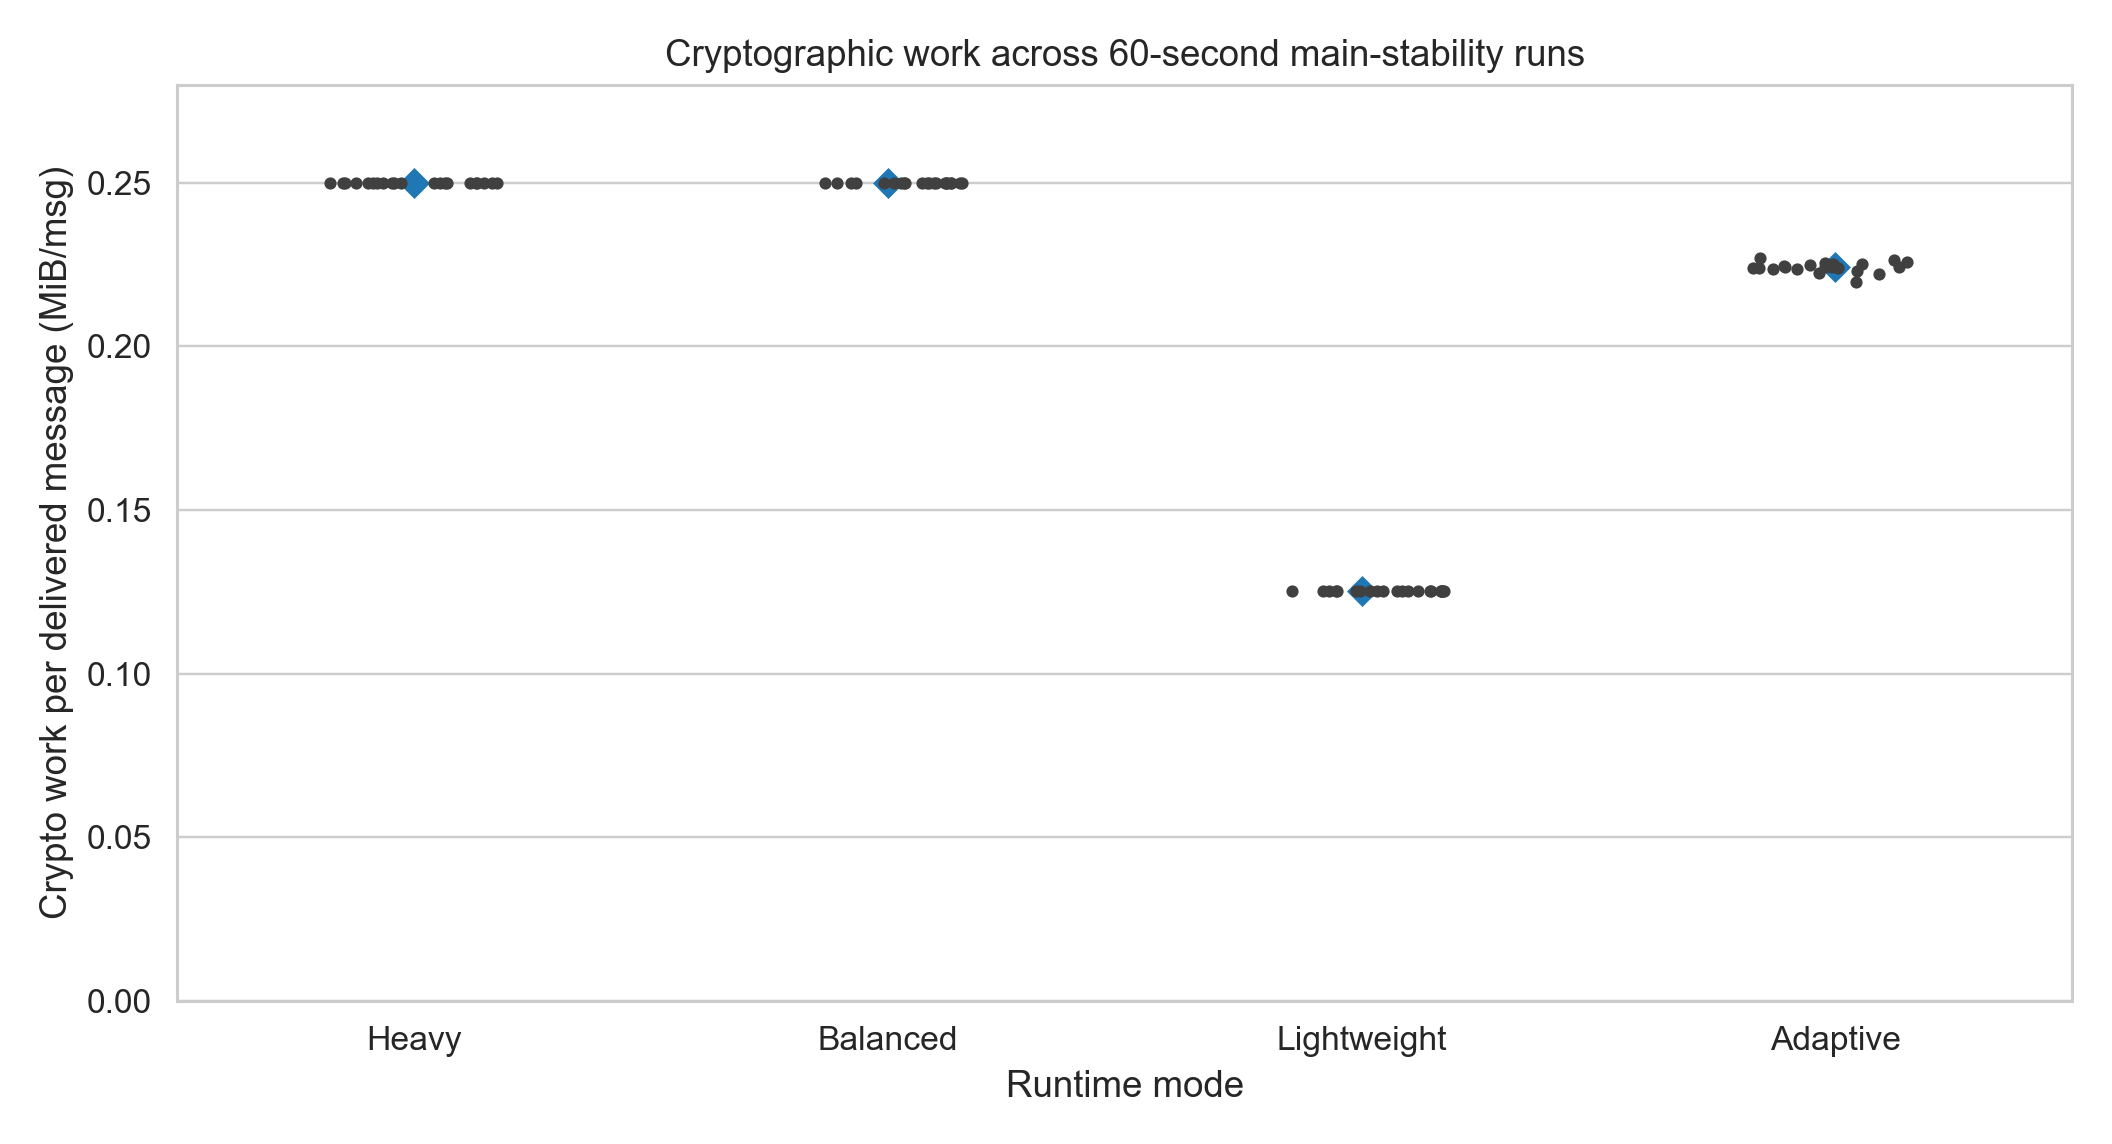
\includegraphics[width=0.86\textwidth]{figs/benchmark_crypto_work_profile.png}
\caption{Long-run cryptographic work across all 60-second main-stability runs; black points are individual runs and blue diamonds are medians.}
\label{fig:benchmark_crypto_work_profile}
\end{figure}

Across the main-stability runs, the median cryptographic work per delivered message is 0.250~MiB for heavy mode, 0.250~MiB for balanced mode, 0.224~MiB for adaptive mode, and 0.125~MiB for lightweight mode. Balanced is not identical to heavy: it uses AES-192-GCM rather than AES-256-GCM. However, the deterministic crypto-work metric counts bytes processed by primitives, not AES round count or key length. Since both heavy and balanced perform one AEAD pass plus one HMAC pass over the same delivered payload, they appear equal in byte-level crypto work. Figure~\ref{fig:benchmark_crypto_work_profile} is therefore the clearest long-run view of primitive-byte workload, while Figure~\ref{fig:benchmark_long_run_policy_tradeoff} shows the ordinal protection-level trade-off. Adaptive is not universally best; it reacts correctly to policy inputs and trades some efficiency for stronger protection during high-threat phases.

Figure~\ref{fig:benchmark_long_run_policy_tradeoff} makes the switching benefit more explicit. It compares four strategies against the same 60-second threat and energy schedule: always-heavy, always-balanced, always-lightweight, and adaptive switching. The middle panel uses protection-tier work rather than wall-clock latency: lightweight contributes one tier-message unit per message, balanced contributes two, and heavy contributes three. This metric is not an energy model; it is an ordinal policy-cost view used to show whether a strategy spends protection budget in the right part of the run.

\begin{figure}[H]
\centering
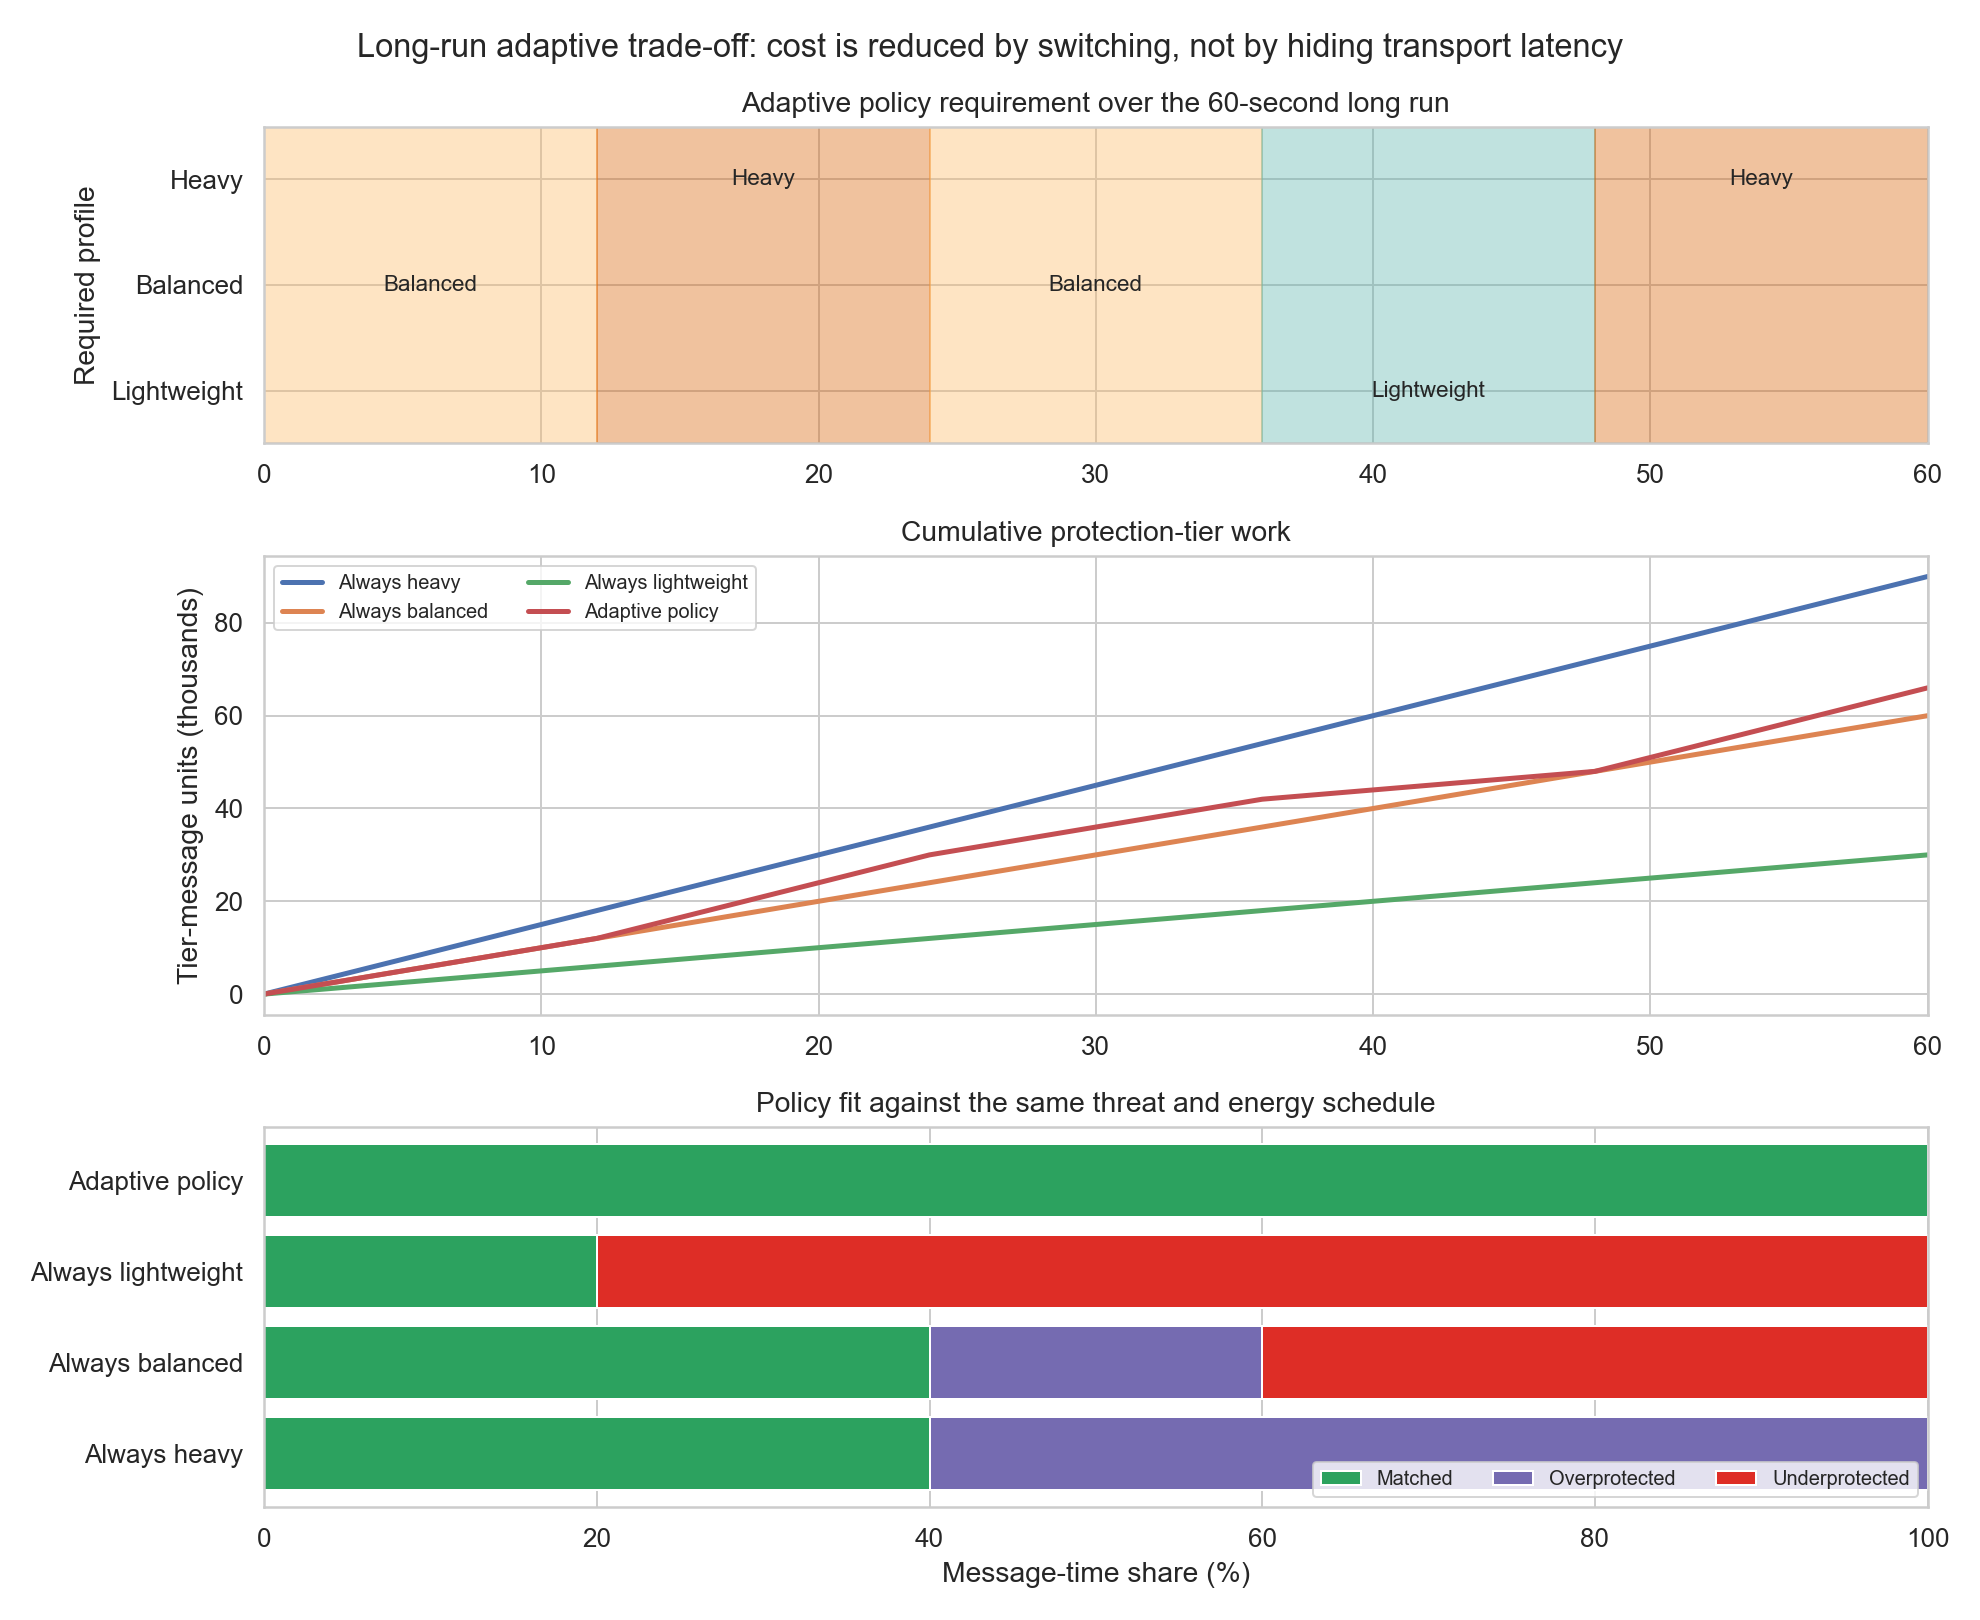
\includegraphics[width=\textwidth]{figs/benchmark_long_run_policy_tradeoff.png}
\caption{Long-run policy trade-off under the scripted threat and energy schedule.}
\label{fig:benchmark_long_run_policy_tradeoff}
\end{figure}

The always-heavy baseline reaches 90 thousand tier-message units and never underprotects, but it overprotects 60\% of the message-time. The always-lightweight baseline uses only 30 thousand tier-message units, but it underprotects 80\% of the message-time. The always-balanced baseline is the static middle point at 60 thousand tier-message units: it matches the balanced portions of the run, but it still underprotects the high-threat windows and overprotects the low-energy window. Adaptive switching reaches 66 thousand tier-message units, saves 26.7\% relative to always-heavy, and matches the required profile for the full schedule. This is the concrete advantage of the balanced/adaptive policy: it is not a large end-to-end latency gap on the host system, but a correct allocation of protection level over time.

\section{Adaptive Switching Behavior}
\label{sec:adaptive_switching}

Adaptive behavior is evaluated both through aggregate metrics and through the recorded switching trace. A representative clean 100~Hz main-stability run recorded four transitions: heavy mode at 12.062 seconds because of high threat, balanced mode at 24.065 seconds when threat fell, lightweight mode at 36.162 seconds under the low-energy condition, and heavy mode again at 48.067 seconds when threat rose. The same run sent 1\,486 heavy-profile messages, 1\,432 balanced-profile messages, and 755 lightweight-profile messages.

Across all 57 adaptive runs, 54 recorded the expected four transitions. The three exceptions are all in the deliberately severe lossy-network profile: two runs recorded zero transitions and one recorded only one transition because the run effectively collapsed under impairment, with sender-side drop rates between 75.566\% and 94.312\%. This is not evidence that the adaptive policy failed under normal conditions; it is evidence that the current containerized transport can become too impaired for the scripted policy timeline to be fully exercised.

\begin{figure}[H]
\centering
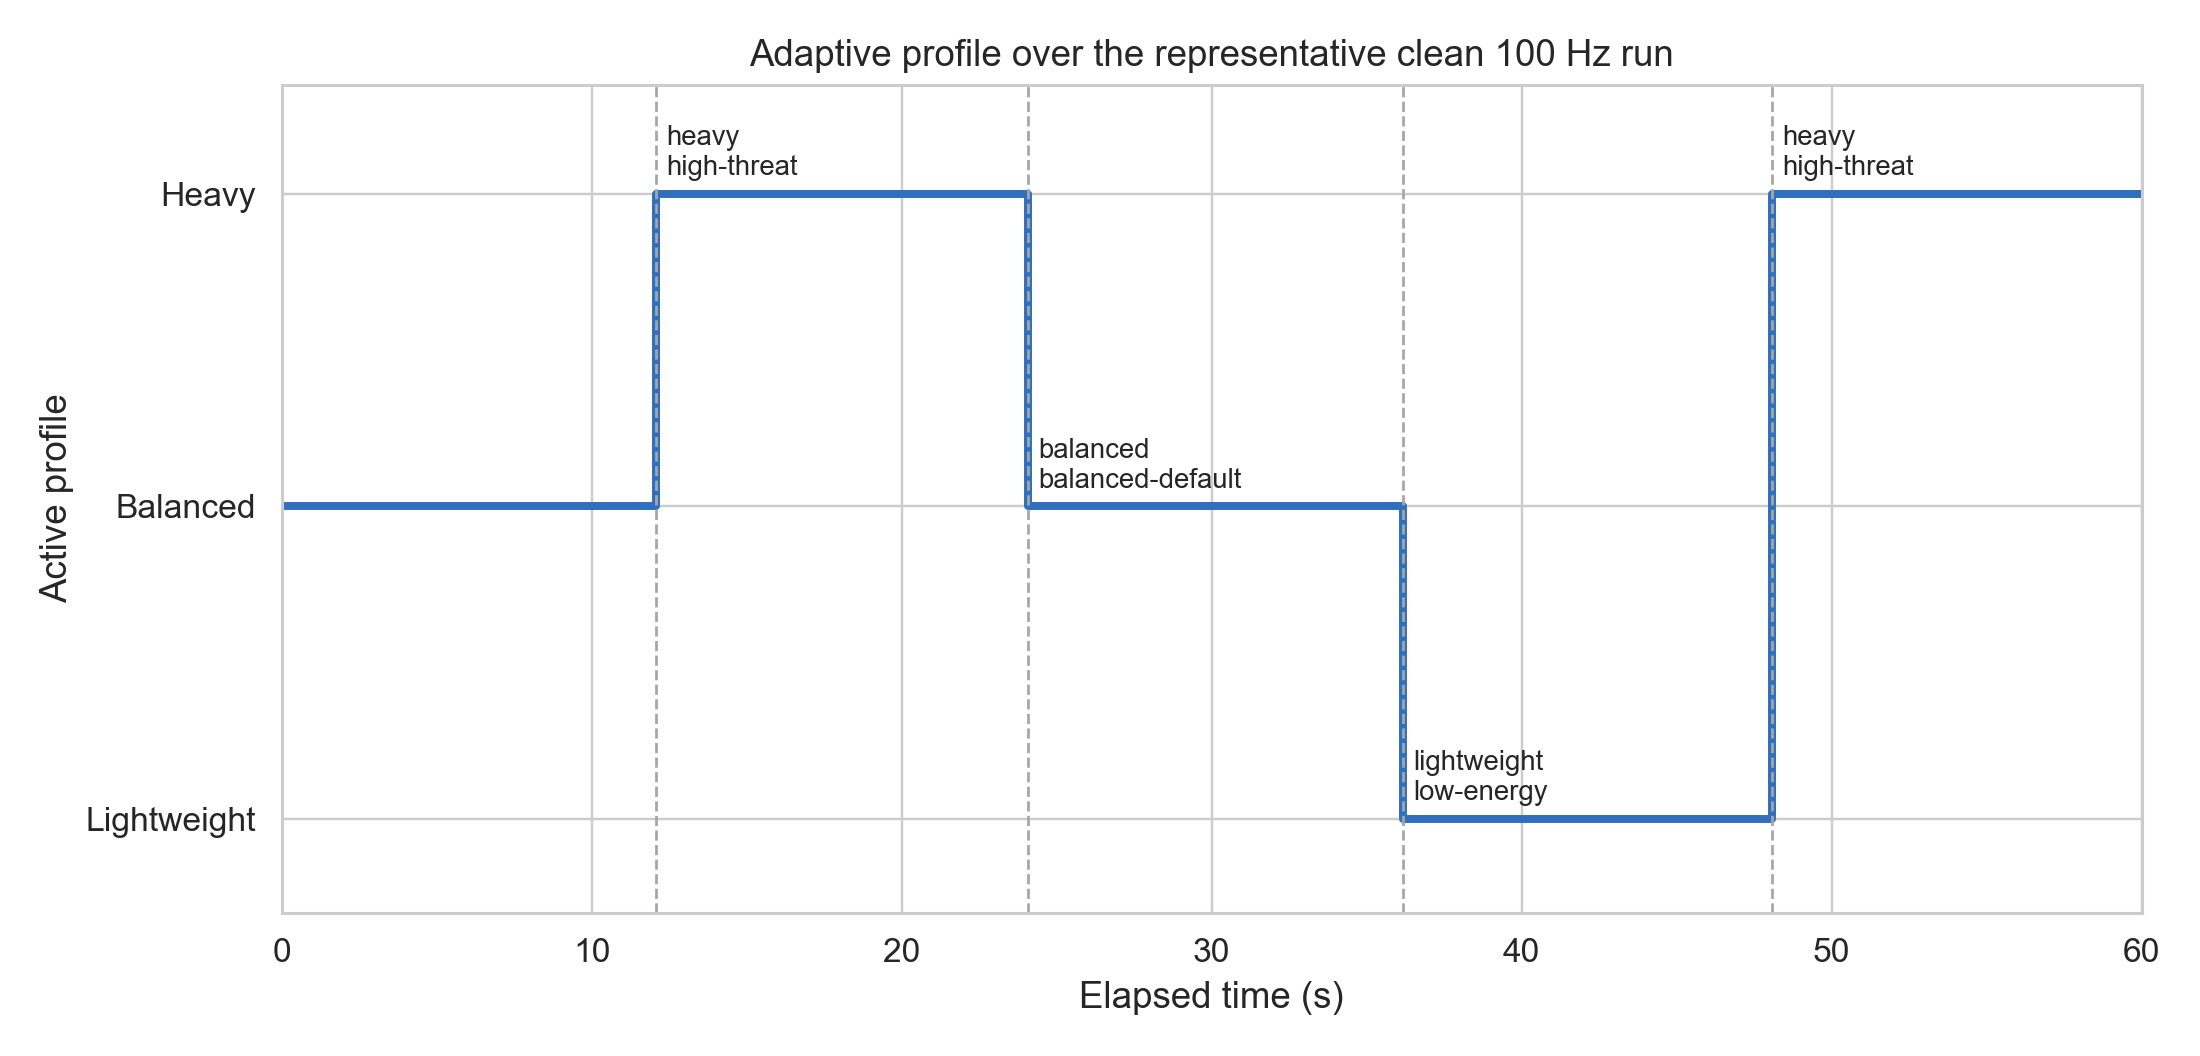
\includegraphics[width=\textwidth]{figs/benchmark_adaptive_switches.png}
\caption{Adaptive switching trace for the representative clean 100~Hz main-stability run.}
\label{fig:benchmark_adaptive_switches}
\end{figure}

\section{Sensitivity Analysis}
\label{sec:sensitivity_analysis}

The final evidence pass includes three targeted sensitivity checks: CPU cap, rekey interval, and network impairment. Table~\ref{tab:cpu_sensitivity} reports the stressed 200~Hz CPU-sensitivity subset. The 100~Hz CPU-sensitivity runs show the same qualitative behavior: CPU caps of 0.10 and 0.25 cores remove the drop observed at 0.05 cores.

\begin{table}[H]
\centering
\small
\caption{CPU sensitivity at 200~Hz; crypto work is in MiB per delivered message}
\label{tab:cpu_sensitivity}
\renewcommand{\arraystretch}{1.15}
\resizebox{\textwidth}{!}{%
\begin{tabular}{|c|l|c|c|c|c|}
\hline
\textbf{CPU cap} & \textbf{Mode} & \textbf{Med. P50} & \textbf{Med. throughput} & \textbf{Med. drop \%} & \textbf{Med. crypto work} \\
\hline
0.05 & Heavy & 198.387 & 60.5 & 68.860 & 0.2500 \\
0.05 & Balanced & 103.972 & 65.7 & 66.832 & 0.2500 \\
0.05 & Lightweight & 194.513 & 69.8 & 64.612 & 0.1251 \\
0.05 & Adaptive & 195.289 & 76.4 & 61.585 & 0.2265 \\
0.10 & Heavy & 97.266 & 147.7 & 26.002 & 0.2500 \\
0.10 & Balanced & 96.721 & 151.9 & 23.930 & 0.2500 \\
0.10 & Lightweight & 97.791 & 151.2 & 24.204 & 0.1251 \\
0.10 & Adaptive & 96.506 & 155.4 & 21.873 & 0.2252 \\
0.25 & Heavy & 1.062 & 200.0 & 0.000 & 0.2500 \\
0.25 & Balanced & 1.156 & 200.0 & 0.000 & 0.2500 \\
0.25 & Lightweight & 1.138 & 200.0 & 0.000 & 0.1251 \\
0.25 & Adaptive & 1.093 & 200.0 & 0.000 & 0.2250 \\
\hline
\end{tabular}
}
\end{table}

\begin{figure}[H]
\centering
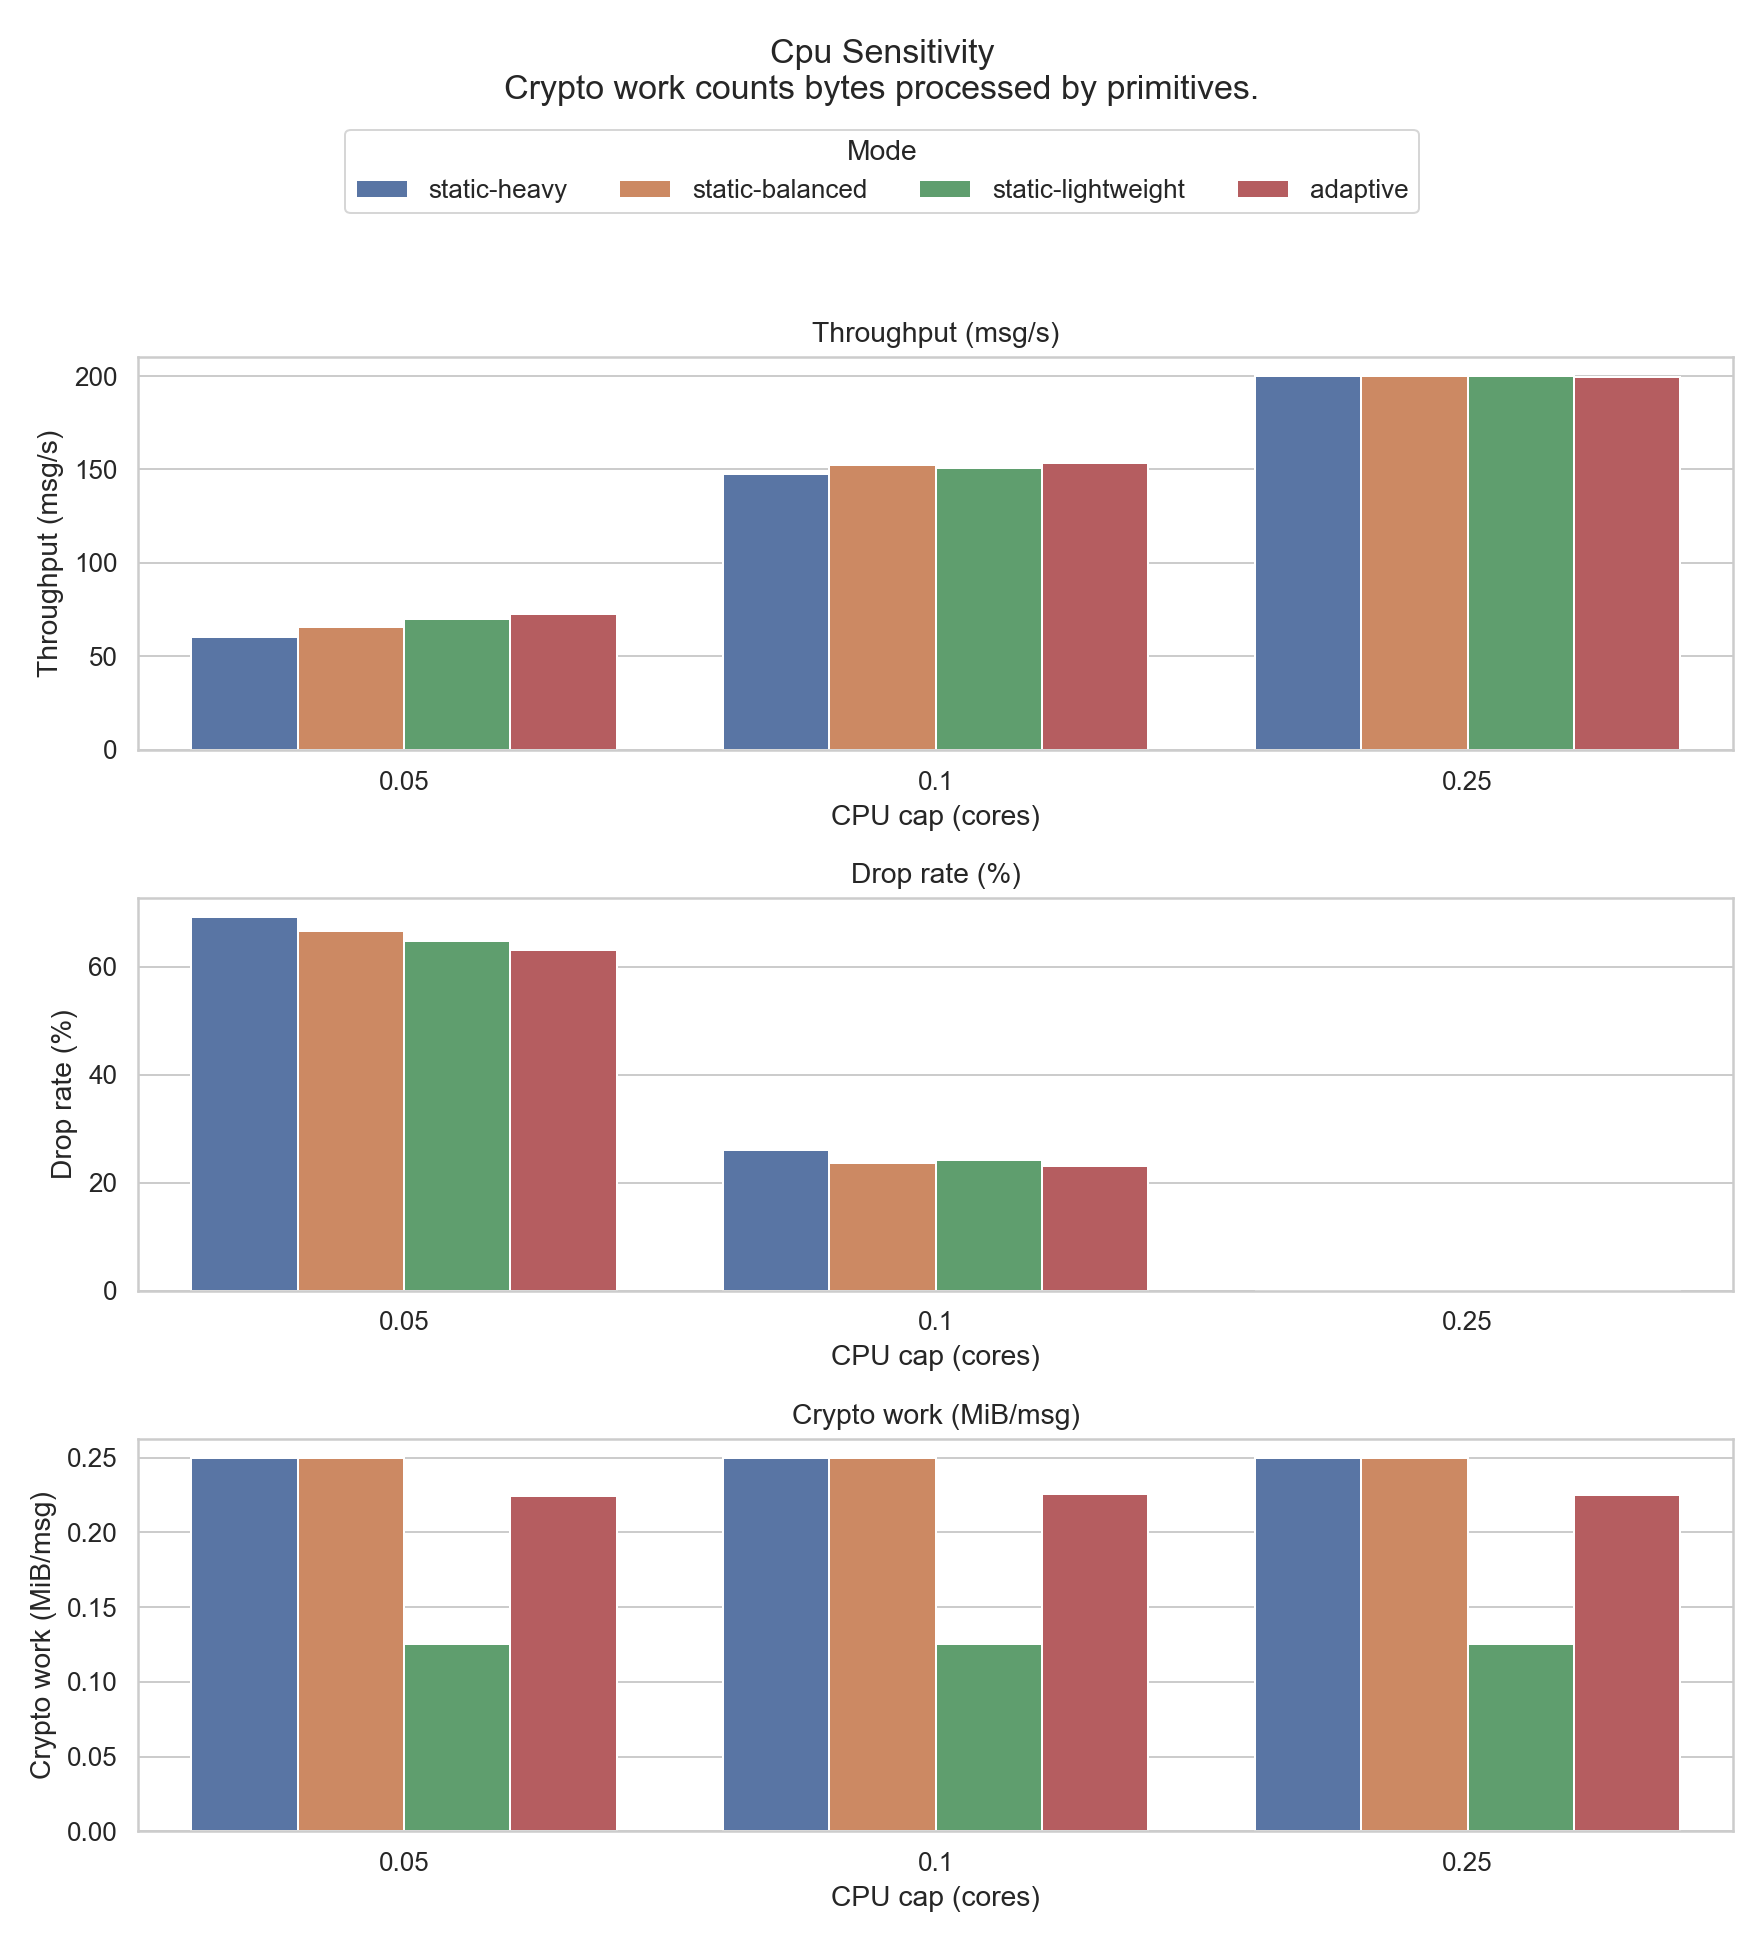
\includegraphics[width=\textwidth]{figs/benchmark_cpu_sensitivity.png}
\caption{CPU sensitivity at 200~Hz: throughput, drop rate, and cryptographic work.}
\label{fig:benchmark_cpu_sensitivity}
\end{figure}

The CPU sensitivity result is the strongest explanation for the saturation behavior. Under the 0.05-core cap, the prototype cannot sustain 200 messages per second and drops roughly 62--69\% of attempted sends. At 0.10 cores the same workload improves substantially but still drops about 22--26\%, while at 0.25 cores it is sustained cleanly in all four modes. This supports the conclusion that the main sweep is CPU-limited rather than limited by the nominal cryptographic design alone. The cryptographic-work panel remains separated because it counts profile-specific primitive work rather than shared end-to-end queueing delay.

Table~\ref{tab:rekey_sensitivity} shows the rekey-interval sensitivity at 100~Hz. In this benchmark pass, changing the rekey interval does not dominate the result: all rows remain close to the same queueing boundary under the 0.05-core cap. This makes the rekey experiment a stability check rather than evidence that a longer interval alone solves the throughput bottleneck.

\begin{table}[H]
\centering
\small
\caption{Rekey sensitivity at 100~Hz and 0.05 CPU cores; crypto work is in MiB per delivered message}
\label{tab:rekey_sensitivity}
\renewcommand{\arraystretch}{1.15}
\resizebox{\textwidth}{!}{%
\begin{tabular}{|c|l|c|c|c|c|}
\hline
\textbf{Rekey interval} & \textbf{Mode} & \textbf{Med. P50} & \textbf{Med. throughput} & \textbf{Med. drop \%} & \textbf{Med. crypto work} \\
\hline
2s & Heavy & 200.406 & 60.0 & 39.325 & 0.2500 \\
2s & Balanced & 201.038 & 63.0 & 36.983 & 0.2500 \\
2s & Lightweight & 199.882 & 62.2 & 37.833 & 0.1251 \\
2s & Adaptive & 201.078 & 60.8 & 38.151 & 0.2239 \\
5s & Heavy & 120.811 & 62.6 & 36.731 & 0.2500 \\
5s & Balanced & 201.605 & 55.5 & 44.167 & 0.2500 \\
5s & Lightweight & 265.201 & 55.4 & 42.768 & 0.1251 \\
5s & Adaptive & 200.346 & 56.1 & 42.277 & 0.2237 \\
10s & Heavy & 293.734 & 54.4 & 43.858 & 0.2500 \\
10s & Balanced & 204.749 & 54.9 & 44.334 & 0.2500 \\
10s & Lightweight & 199.739 & 55.4 & 43.357 & 0.1251 \\
10s & Adaptive & 201.683 & 55.9 & 43.604 & 0.2237 \\
\hline
\end{tabular}
}
\end{table}

\begin{figure}[H]
\centering
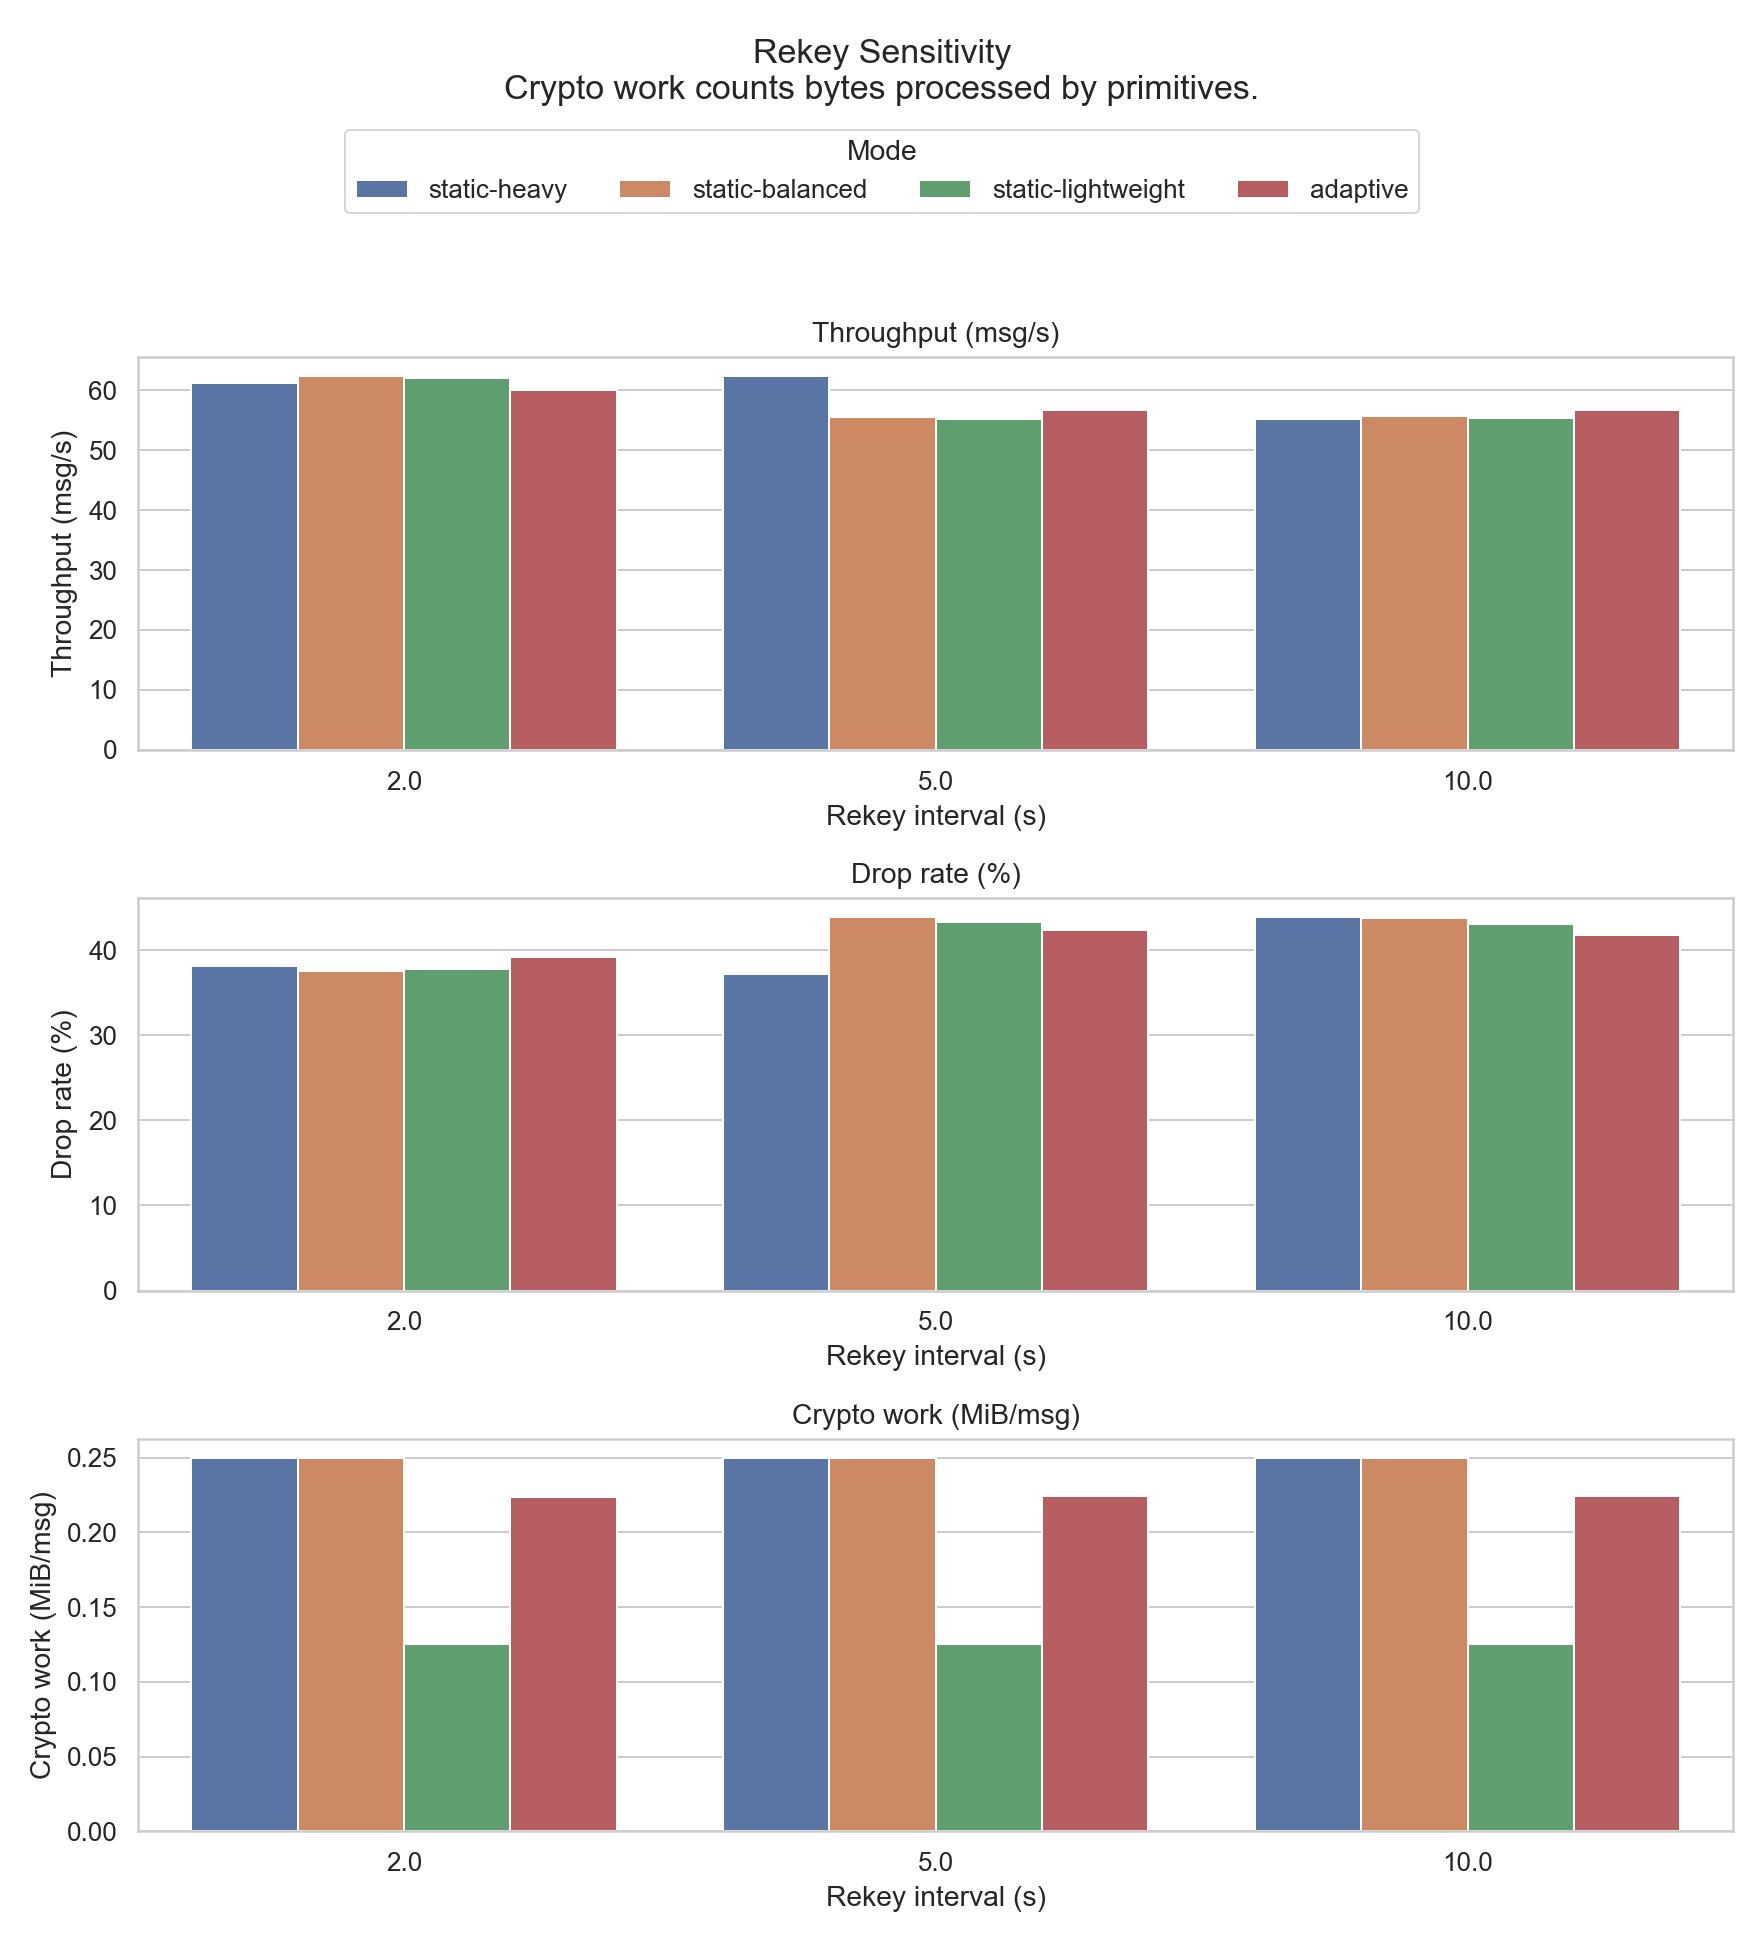
\includegraphics[width=\textwidth]{figs/benchmark_rekey_sensitivity.png}
\caption{Rekey-interval sensitivity at 100~Hz and 0.05 CPU cores, including cryptographic work.}
\label{fig:benchmark_rekey_sensitivity}
\end{figure}

Table~\ref{tab:network_impairment} reports the network-impairment sweep. The clean profile is consistent with the main 100~Hz result. The mild and lossy profiles sharply reduce delivered throughput and increase drop rate, which shows that the benchmark can expose transport-level fragility rather than hiding it behind crypto-only measurements. The impairment profiles jointly vary delay, jitter, and packet loss: clean uses 0/0/0, mild uses 20/5/2, and lossy uses 50/15/5. Figure~\ref{fig:benchmark_network_impairment} uses grouped bars rather than overlaid lines because the intended reading is the network-level collapse from clean to impaired conditions, not a fine-grained profile ordering inside each impaired condition. All 36 network-impairment runs completed, but the lossy rows should still be interpreted as transport collapse under deliberately severe delay, jitter, and packet-loss settings, not as stable steady-state performance of the cryptographic profiles. In these impaired runs, the reported drop rate includes both backlog-induced unsent attempts and explicit send errors observed by the sender.

\begin{table}[H]
\centering
\small
\caption{Network impairment at 100~Hz; crypto work is in MiB per delivered message}
\label{tab:network_impairment}
\renewcommand{\arraystretch}{1.15}
\resizebox{\textwidth}{!}{%
\begin{tabular}{|l|l|c|c|c|c|}
\hline
\textbf{Network} & \textbf{Mode} & \textbf{Med. P50} & \textbf{Med. throughput} & \textbf{Med. drop \%} & \textbf{Med. crypto work} \\
\hline
Clean & Heavy & 199.173 & 56.5 & 42.650 & 0.2500 \\
Clean & Balanced & 200.178 & 52.2 & 47.581 & 0.2500 \\
Clean & Lightweight & 201.536 & 50.9 & 48.637 & 0.1251 \\
Clean & Adaptive & 200.773 & 54.6 & 44.068 & 0.2239 \\
Mild & Heavy & 1575.028 & 11.9 & 87.907 & 0.2500 \\
Mild & Balanced & 1705.948 & 10.6 & 88.523 & 0.2500 \\
Mild & Lightweight & 1195.236 & 13.9 & 85.990 & 0.1251 \\
Mild & Adaptive & 1641.189 & 10.2 & 89.793 & 0.2243 \\
Lossy & Heavy & 2387.132 & 1.1 & 96.924 & 0.2267 \\
Lossy & Balanced & 2034.417 & 0.5 & 99.470 & 0.2348 \\
Lossy & Lightweight & 1000.831 & 1.6 & 84.953 & 0.1180 \\
Lossy & Adaptive & 1045.680 & 1.8 & 85.128 & 0.2126 \\
\hline
\end{tabular}
}
\end{table}

\begin{figure}[H]
\centering
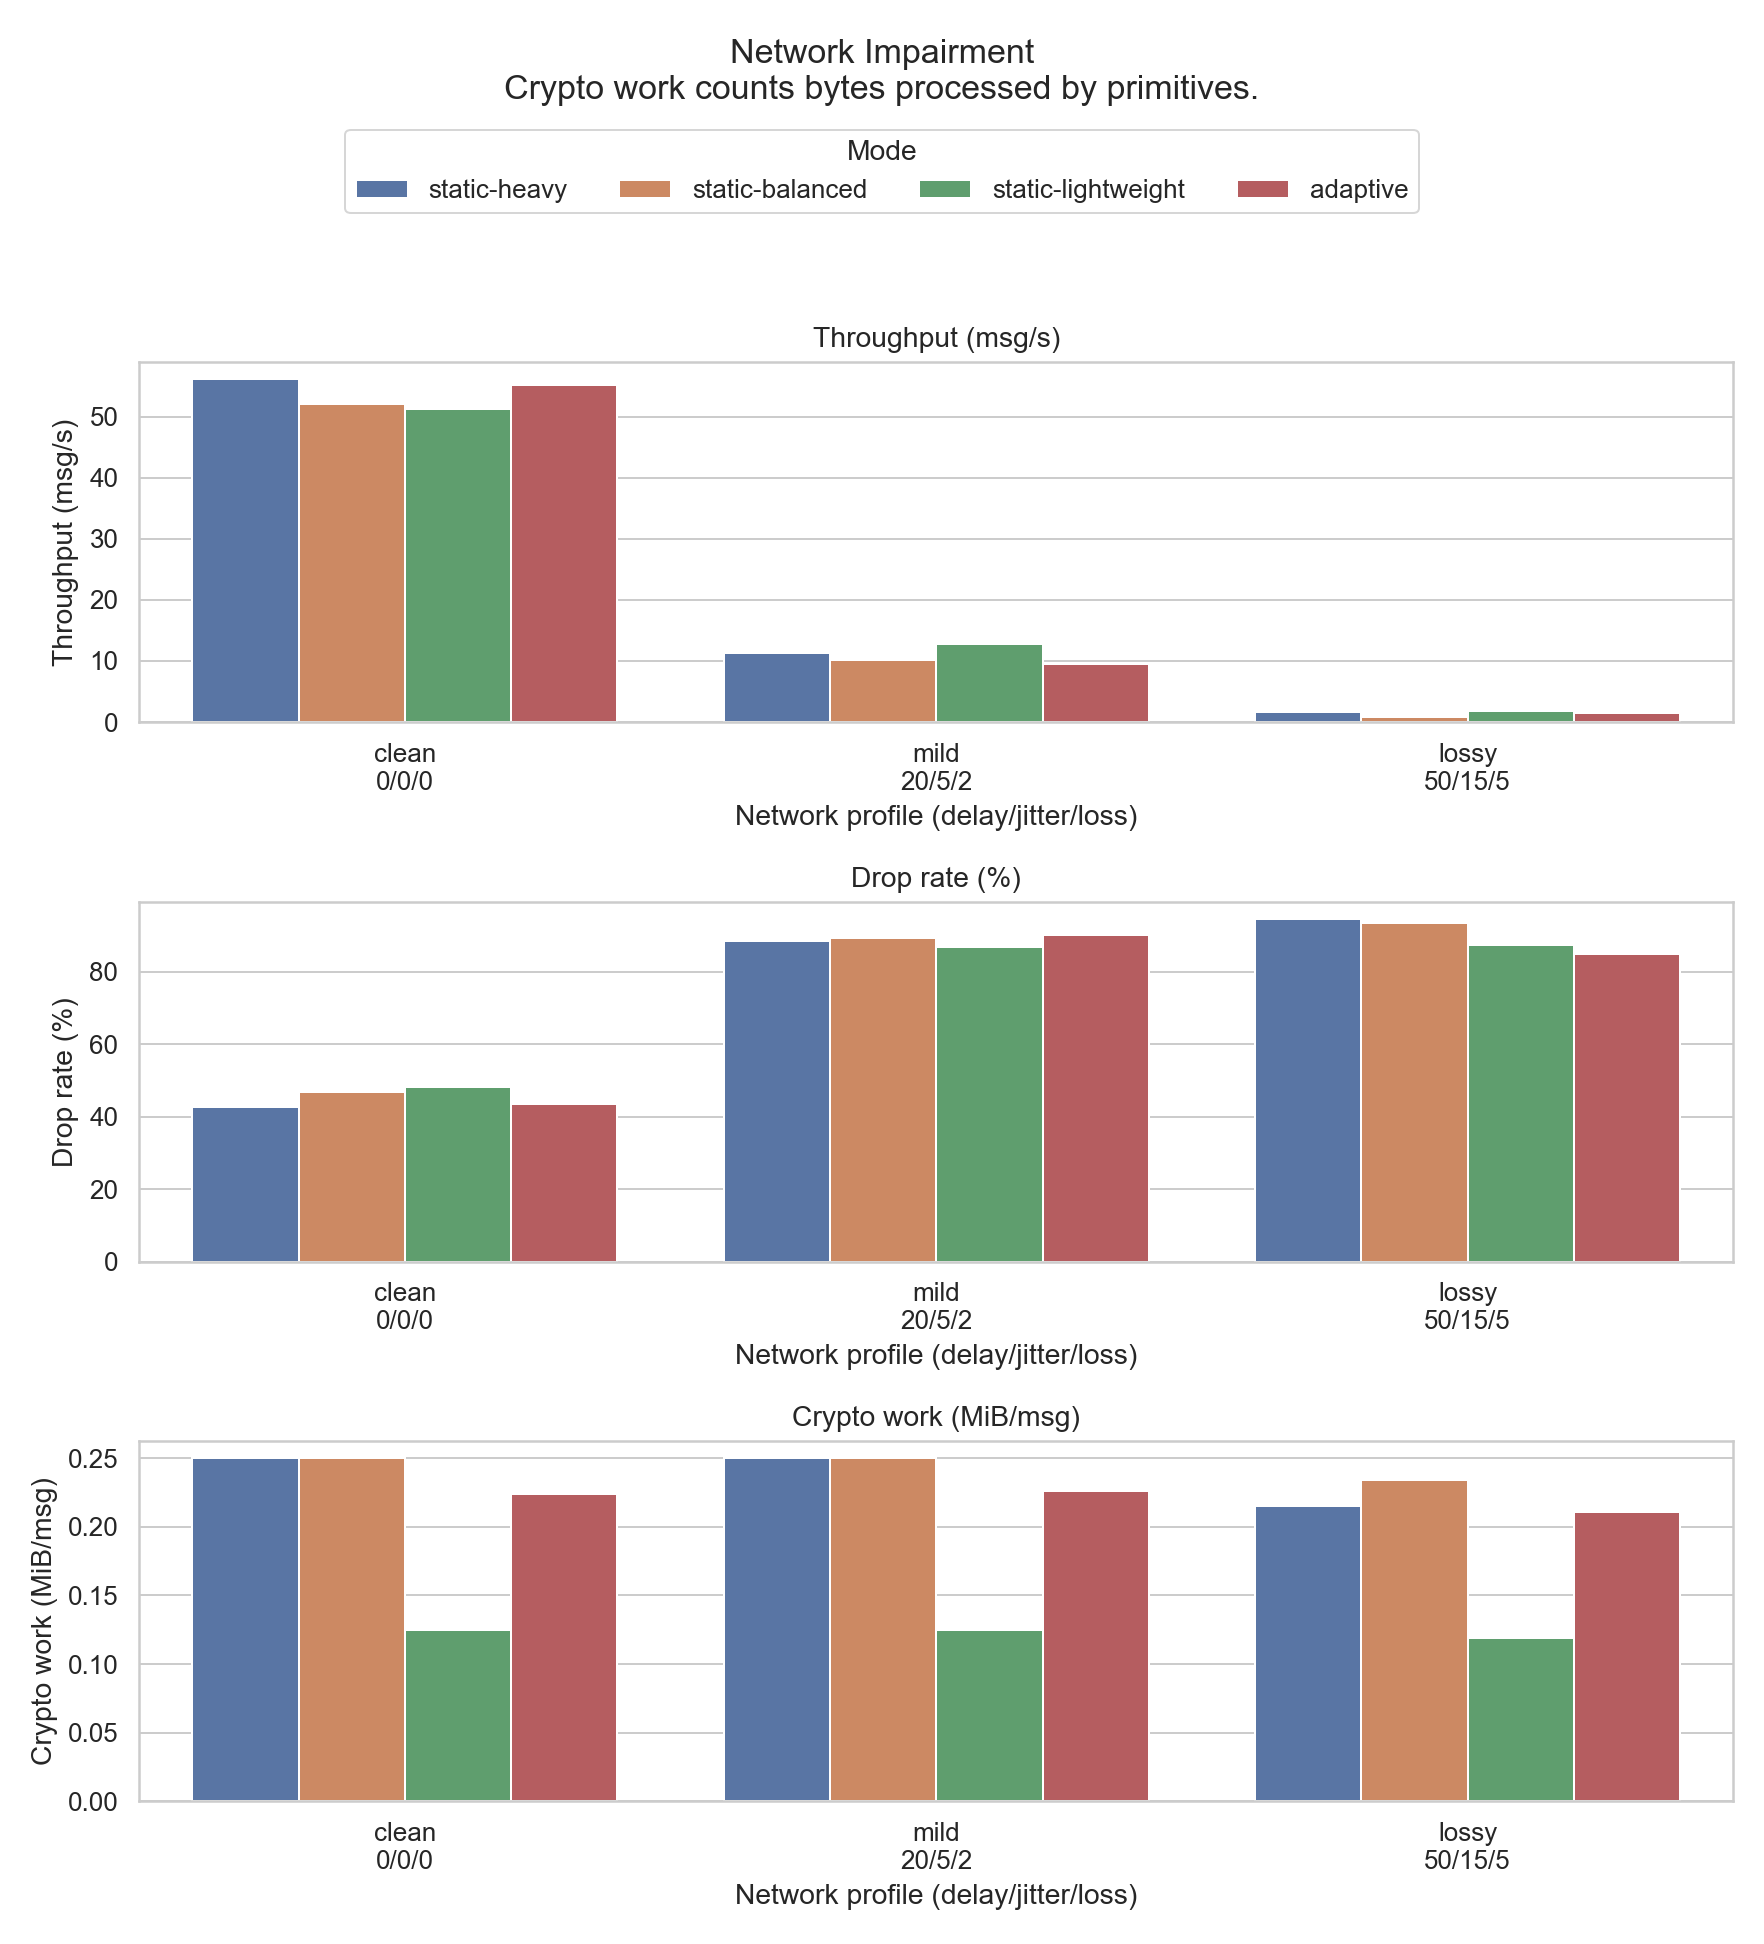
\includegraphics[width=\textwidth]{figs/benchmark_network_impairment.png}
\caption{Network-impairment sensitivity at 100~Hz; profile labels are delay/jitter/loss.}
\label{fig:benchmark_network_impairment}
\end{figure}

\section{Practical Findings}
\label{sec:practical_findings}

The final benchmark results support five practical conclusions.
\begin{itemize}
    \item Lightweight mode is the strongest default among the tested profiles when compute is the dominant constraint and maximum protection is not required at every instant: it has the lowest cryptographic work per delivered message and generally the highest sustained throughput in the repeated main sweep.
    \item Adaptive mode behaves correctly as a policy-driven compromise: it reacts to scripted runtime conditions and trades efficiency for stronger protection during high-threat periods. It should not be described as universally best.
    \item Heavy and balanced modes remain relevant authenticated operating points, but their HMAC authentication pass shows up as consistently higher cryptographic work per delivered message than lightweight mode.
    \item Offered-load experiments must be interpreted through attempted rate, delivered throughput, and drop rate together. Under the strict CPU cap, higher nominal offered rates mostly increase backlog and drops rather than proving linear scaling.
    \item Close end-to-end curves are not evidence that the benchmark is uninformative. They show that, for this containerized long-run setup and 65\,536-byte messages, transport and CPU scheduling dominate measured latency once the system is near saturation.
\end{itemize}

These findings are stronger than purely analytical estimates because they are tied to executable artifacts and repeated runs. They remain narrower than a field study. The practical evaluation validates a constrained pairwise prototype running in containers, not a complete multi-hop or large-swarm secure-communication stack, and the energy metric remains a model-based proxy rather than a physical power measurement. The cryptographic-work metric is not a power measurement either, but it is derived from raw execution counters rather than chosen energy coefficients.
